\section {PlanesWidget}

\subsection{MainWindow}

The GUI is hosted by a QMainWindow of the derived class PlanesWWindow. The constructor of PlanesWWindow creates the game controller (a PlaneRound object) and gives it as parameter to the central area of the QMainWindow, which is an object of the class PlanesWView.


\begin{lstlisting}
PlanesWWindow::PlanesWWindow(QWidget *parent) :
	QMainWindow(parent)
{
	//builds the game object - the controller
	mRound = new PlaneRound(10, 10, 3);
	
	//builds the view object
	mPlanesView = new PlanesWView(mRound);
	setCentralWidget(mPlanesView);
	
	//starts the game
	mRound->initRound();
}

\end{lstlisting}

PlanesWView creates in the constructor the layout of the GUI. In Figure \ref{fig:planeswidget_game_widgetnames} are shown the names of the widgets used in the game area layout.

\begin{figure}[h]
	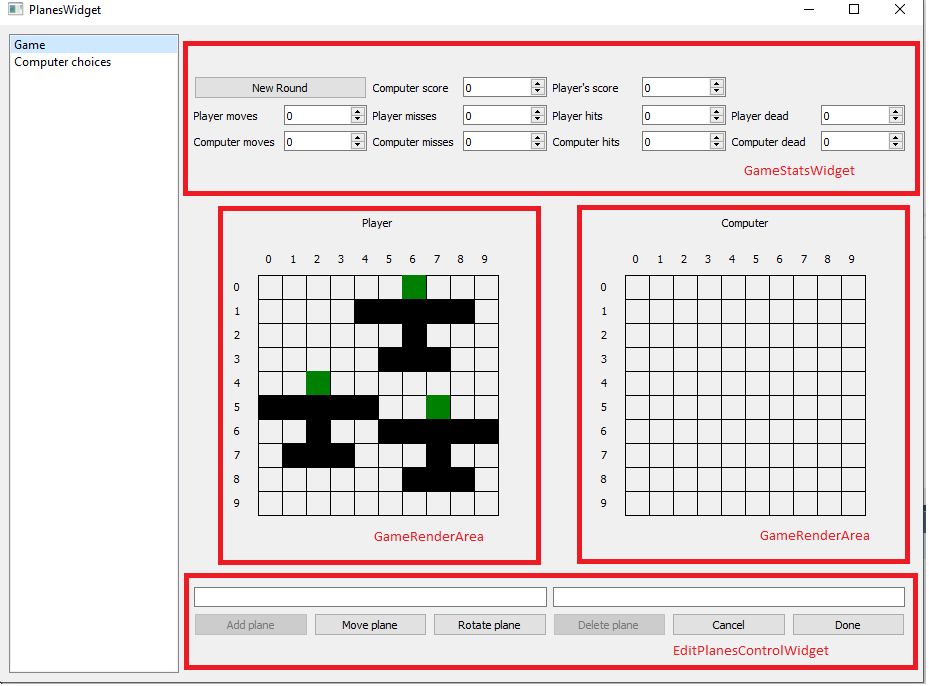
\includegraphics[width = \textwidth]{PlanesWidget_Game_WidgetNames.png}
	\caption{Widgets in the game area layout}
	\label{fig:planeswidget_game_widgetnames}
\end{figure}

It is relevant to see the member variables of PlanesWView:

\begin{lstlisting}
	//PlaneGrid objects manage the logic of a set of planes on a grid
	//as well as various operations: save, remove, search, etc.
	PlaneGrid* m_playerGrid;
	PlaneGrid* m_computerGrid;
	
	//GameRenderArea objects are graphical objects that
	//display guesses, computer choices , planes
	//in grids
	GameRenderArea* m_playerArea;
	GameRenderArea* m_computerArea;
	
	//EditPlanesControlWidget is a widget that controls the
	//process of planes positioning and adding in the
	//player grid
	EditPlanesControlWidget* m_editPlanesWidget;
	
	//GameStatsWidget displays the statistics about the current
	//game and about the score
	GameStatsWidget* m_gameStatsWidget;
	
	//ChoiceDebug window is a widget that shows how the
	//computer plays
	ChoiceDebugWidget* m_choiceDebugWidget;
	
	//ComputerLogic is the object that keeps the
	//computer's strategy
	ComputerLogic* m_computerLogic;
	
	//PlaneRound is the object that coordinates the game
	PlaneRound* m_round;
\end{lstlisting}

The PlaneRound object is given to the PlanesWView as constructor parameter. In the constructor of PlanesWView the pointers to the 2 PlanesGrids and the ComputerLogic objects are read from the PlaneRound object. Based on these objects the 4 main widgets of the game interface: the 2 GameRenderArea, the GameStatsWidget and the EditPlanesControlWidget are created.

GameStatsWidget and EditPlanesControlWidget are created based on graphically defined layouts EditControl.ui and GameForm.ui, which use a xml format to save the position of the elements of each layout.

The two GameRenderArea, m\_playerArea and m\_computerArea, display the game boards of computer and player.


\subsection{BaseRenderArea}

BaseRenderArea is the basis class for GameRenderArea, which display the player's game board or the computer's game board. 

It derives from QWidget, the basis class for all widgets in Qt. In order to display the game board it overrides the paintEvent() function of QWidget. 

In the paintEvent() function the vertical and horizontal lines of the board are drawn as well as the line numbers.

The board game is drawn centered inside the widget space allocated for the widget by the layout.

The class implements a method called drawGuesses() which displays the guesses made by the computer or player.

\subsection{GameRenderArea}

\subsection{Connections Between Widgets}

The interaction between different widgets is accomplished by using Qt's signal and slots mechanismus \ref{Qt_Signals_Slots}. 


\subsection {Qt Concepts}

\subsubsection{Signal and Slots Mechanismus} \label {Qt_Signals_Slots}

One of the main features of Qt is a communication mechanism named "signal-slots". It allows communication between objects deriving from the Qt class QObject. A signal is a function returning void declared in a special section of the class declaration. The QObject declaring the signals can call the signal-functions with a special syntax. QObjects wishing to be notified when the signal-functions are called define and declare matching special functions called "slots". These functions are to be executed in response to signals. Pairing of signals and slots occurs outside the concerned objects, maybe in a class which has the two QObjects as member variables. It is required that the parameters of the paired signals and slots to be of the same type. Thus parameters can be transmitted from the emitter object to the receiver object when a signal is emitted and the corresponding slot is executed. 

The example code below is from the PlanesWView constructor:

\begin{lstlisting}
    connect(m_playerArea, SIGNAL(operationEndet()),
		m_editPlanesWidget, SLOT(cancel_clicked()));
	connect(m_playerArea,SIGNAL(displayMsg(QString)),
		m_editPlanesWidget, SLOT(displayMsg(QString)));
	connect(m_playerArea, SIGNAL(enoughPlanes()),
		m_editPlanesWidget, SLOT(deactivateAddPlane()));
	connect(m_playerArea, SIGNAL(displayStatusMsg(const std::string&)),
		m_editPlanesWidget, SLOT(displayStatusMsg(const std::string&)));
	connect(m_playerArea, SIGNAL(notEnoughPlanes()),
		m_editPlanesWidget, SLOT(deactivateDoneButton()));
	connect(m_playerArea, SIGNAL(activateDone()),
		m_editPlanesWidget, SLOT(activateDoneButton()));
	connect(m_playerArea, SIGNAL(deactivateDone()),
		m_editPlanesWidget, SLOT(deactivateDoneButton()));
	connect(m_editPlanesWidget, SIGNAL(doneClicked()),
		m_playerArea, SLOT(changeMode()));
	connect(m_editPlanesWidget, SIGNAL(doneClicked()),
		this, SLOT(doneClicked()));

	connect(m_computerArea, SIGNAL(guessMade(const GuessPoint&)),
		this, SLOT(receivedPlayerGuess(const GuessPoint&)));
	connect(m_gameStatsWidget, SIGNAL(startGame()),
		this, SLOT(startNewRound()));
	
	connect(listWidget, SIGNAL(currentRowChanged(int)),
		stackedLayout, SLOT(setCurrentIndex(int)));
	connect(listWidget, SIGNAL(currentRowChanged(int)),
		this, SLOT(widgetSelected(int)));
	connect(this, SIGNAL(debugWidgetSelected()),
		m_choiceDebugWidget, SLOT(setLogic()));
\end{lstlisting}

\subsubsection{Layouts}

In contrast to the EditPlaneControlWidget and GameStatsWidget where the layout is created with a graphic editor, the layout of the PlanesWView is created programmatically:

\begin{lstlisting}


	//builds the layout for this view
	QSplitter* hsplitter = new QSplitter(Qt::Horizontal);
	hsplitter->addWidget(m_playerArea);
	hsplitter->addWidget(m_computerArea);
	
	QSplitter* vsplitter = new QSplitter(Qt::Vertical);
	vsplitter->addWidget(m_gameStatsWidget);
	vsplitter->addWidget(hsplitter);
	vsplitter->addWidget(m_editPlanesWidget);
	
	QListWidget *listWidget = new QListWidget;
	listWidget->addItem(tr("Game"));
	listWidget->addItem(tr("Computer choices"));
	
	QFontMetrics fm = listWidget->fontMetrics();
	int maxWidth = fm.width("Computer choices");
	listWidget->setFixedWidth(maxWidth * 2);
	
	QStackedLayout* stackedLayout = new QStackedLayout;
	stackedLayout->addWidget(vsplitter);
	stackedLayout->addWidget(m_choiceDebugWidget);
	
	listWidget->setCurrentRow(0);
	
	QHBoxLayout* mainLayout = new QHBoxLayout();
	mainLayout->addWidget(listWidget);
	mainLayout->addLayout(stackedLayout);
	
	setLayout(mainLayout);

\end{lstlisting}

A QSplitter is a widget which shows the containing widgets one next to the other or one under the other depending on the given orientation at object construction. A QStackedLayout is a layout that shows only one of many owned widgets at a time. So the hsplitter contains the two game boards arranged horizontally, the vsplitter contains the GameStatsWidget, vsplitter and the EditPlanesControlWidget arranged vertically. Then in a QStackedLayout we add two widgets: the vsplitter and another widget, used for debugging.

Finally we come to the main layout of the widget which is called mainLayout and isa QHBoxLayout. A QHBoxLayout places the owned widgets one next to the other in the layout. We assigne the PlanesWView widget this main layout with the function call: setLayout(mainLayout).

The code above is an example of using layouts. The principle is to create the widgets and a layout object (e.g. QHBoxLayout), then add the widgets to the layout with the addWidget() function call. It is possible to add a layout to another layout with the function addLayout(). The topmost layout in the layout hierarchy is then set to the target widget with the function setLayout().